\documentclass[10pt,twocolumn]{article}
\usepackage[a4paper,margin=18mm,columnsep=6mm]{geometry}
\usepackage[utf8]{inputenc}
\usepackage[T1]{fontenc}
\usepackage[spanish]{babel}
\usepackage{graphicx,booktabs,amsmath,url,hyperref}
\graphicspath{{figuras/}{deliveries/week12/paper/figuras/}}
\hypersetup{colorlinks=true,urlcolor=blue,linkcolor=blue}
\title{Fractal: demanda, conexiones y ritmos del subway de Nueva York}
\author{Renzo Acervo Correa \and Stewart Maquera Bobadilla \and José Condori Palomino}
\date{DS5343 Data Visualization, UTEC, 2026-2\\Borrador revisado: 28 de octubre de 2026}
\begin{document}\maketitle
\begin{abstract}
Presentamos un panel exploratorio para estudiar intensidad, distribución semanal y relaciones territoriales del subway. Combinamos entradas estimadas de 2019--2024 con OD estimado de 2021--2024 y caminos asignados a una red GTFS de referencia 2026. Un mapa con abstracción inspirada en RAEB se coordina con una dispersión volumen--forma y un reloj semanal. Separamos datos publicados, caminos modelados y geometría visual. Formulamos seis tareas distintas y preparamos evidencia reproducible, sin presentar todas como interacciones terminadas. Los resultados territoriales ilustran que perder volumen y ganar participación pueden coexistir. La evaluación con usuarios y la integración de algunos detalles analíticos siguen pendientes.
\end{abstract}
\begin{figure}[h]\centering\small
\fbox{\parbox{.91\columnwidth}{Entradas 2019--2024 $\rightarrow$ semanas comparables\\OD 2021--2024 + GTFS 2026 $\rightarrow$ caminos asignados\\$\downarrow$ normalización, agregación, validación\\Mapa enlazado + volumen/forma + reloj semanal\\$\downarrow$ selección, detalle y evidencia exportable}}
\caption{Resumen del procesamiento. La abstracción del mapa no modifica la demanda ni crea enlaces del grafo.}
\end{figure}
\section{Problema y audiencia}
Un total de entradas no distingue redistribución territorial, cambios de horario ni relaciones entre zonas. Analistas de transporte e investigadores urbanos necesitan identificar lugares y franjas para aforos, revisión de demanda y estudios de contingencia. Periodistas de datos son una audiencia secundaria. La contribución es una experiencia integrada y reproducible, no un modelo de frecuencias óptimas ni una explicación causal del COVID.
\section{Preguntas y abstracción de tareas}
Siguiendo la separación entre propósito, medios y entradas/salidas de Brehmer y Munzner~\cite{tasks}, definimos seis resultados diferentes. T1 compara demanda y participación territorial entre 2019 y 2024. T2 compara composición de destinos y dependencia de Manhattan durante 2021--2024. T3 identifica ventanas temporales de demanda. T4 resume carga OD asignada y aportes territoriales por tramo. T5 compara orígenes y destinos externos de un territorio. T6 produce escenarios de retirada de un enlace, con demanda fija, y compara desconexión y desvío.
Las consultas combinan explorar, localizar, identificar, comparar y resumir. Zoom, bundling, selección y exportación son medios transversales, no tareas adicionales. Cada pregunta tiene cantidades y criterios verificables en el repositorio. Tener esos cálculos no implica que todos estén integrados en la interfaz.
\section{Trabajo relacionado}
RAEB~\cite{raeb} usa jerarquía de rutas y abstracción graduable para conciliar simplificación y contexto de red. KDEEB~\cite{kdeeb} informa estimación de densidad, advección y suavizado; nuestra implementación WebGPU requiere validación propia. Dhont et al.~\cite{clock} documentan huellas de siete anillos y 24 sectores y su resta. Gleicher et al.~\cite{comparison} distinguen yuxtaposición, superposición y diferencias explícitas; Shneiderman~\cite{mantra} informa el recorrido de exploración.
Fredriksson y Karlström~\cite{tv} utilizan variación total para comparar repartos modales. Adaptamos la fórmula a 168 celdas semanales; el artículo no demuestra que sea la métrica óptima para este problema. Las demos MBTAViz y Tube Heartbeat orientan coordinación y lectura geográfica, sin importar datos operativos que no poseemos.
\section{Datos y transformaciones}
Las entradas MTA/Open NY cubren 72 meses de 2019--2024, con 141.836.156 registros y 12 campos originales. El OD estimado cubre 48 meses de 2021--2024, con 446.399.011 registros y 16 campos. La visualización usa 424 complejos de subway; otros modos presentes en los originales se contabilizan aparte. La red estática deriva de GTFS 2026: 547 enlaces ferroviarios y dos transferencias peatonales declaradas. No se añaden conexiones por proximidad. Borough y NTA 2020 agrupan complejos por ubicación, no por domicilio de pasajeros.
Para el promedio mensual OD $a_{ymdh oj}$, con $n_{ymd}$ ocurrencias del día semanal, construimos
\[q_{ydh oj}=\frac{\sum_m n_{ymd}a_{ymdh oj}}{\sum_m n_{ymd}}.\]
La suma de destinos produce cantidades iniciadas $u_{odh}$. La semana representativa tiene un lunes, un martes, etc.; $V=\sum_{dh}u_{dh}$ y $p_{dh}=u_{dh}/V$. Para entradas se suman registros y se divide por ocurrencias anuales de cada día. Nunca se resta un perfil de entradas a un perfil OD.
El índice de volumen es $100V_1/V_0$ y el cambio de forma es $TV_{pp}=50\sum_{dh}|p_1-p_0|$. La diferencia de una celda es $100(p_1-p_0)$ en pp. Volumen nulo impide normalizar; base cero deja el índice indefinido. Los grupos suman cantidades antes de normalizar. Una ausencia dentro de meses completos se trata según el supuesto declarado; un mes faltante impide la preparación.
\subsection{Relaciones, carga y escenarios}
La matriz territorial $F_{RS}=\sum_{o\in R,j\in S,dh}q_{dh oj}$ conserva la demanda total. Sus filas normalizadas describen composición de destinos; cantidad y participación se presentan juntas. La carga de un enlace es $L_e=\sum_{oj}q_{oj}\mathbf1[e\in P_{oj}]$, para caminos por distancia sobre la red de referencia. Un viaje puede aportar a varios enlaces; su suma no es un total de personas.
El balance externo es $B_R=(D_R-O_R)/(D_R+O_R)$, excluyendo viajes internos y mostrando ambas cantidades. Destinos agrupados por hora de origen no son salidas observadas a esa hora.
T6 retira ambos sentidos disponibles de un enlace ferroviario identificado. Para pares distintos previamente conectados, calcula demanda que pierde conexión y distancia adicional ponderada entre quienes conservan un camino. Se mantienen denominadores separados. Se prepararon seis ejemplos, no un ranking exhaustivo; se controla que retirar enlaces no acorte caminos mínimos y que la demanda se conserve. No se modelan demoras, oferta ni adaptación de viajeros.
\section{Diseño e implementación}
Un mapa dominante, dispersión superior derecha, reloj inferior derecho y minimapa mantienen contexto en un panel. D3 gestiona geometría, cámara, marcas SVG, selección y vistas enlazadas. WebGPU refina muestras y rasteriza curvas; existe respaldo CPU/WebGL2. Se usan artefactos agregados y 672 matrices comprimidas, sin enviar los originales completos al navegador.
El área del nodo codifica viajes iniciados por cohorte. Agrupación y fidelidad son parámetros visuales entre cero y uno: el primero regula atracción y el segundo conservación de la jerarquía de referencia. Con fidelidad cero hay abstracción libre; con uno se recupera geometría GTFS. Los cruces visuales no crean vías ni transbordos. La fusión de bandas usa peso óptico local y saturación; su ancho no permite leer carga exacta por corredor.
La dispersión codifica índice de volumen y TV mediante posición. El reloj asigna anillo a día, ángulo a hora y color divergente a cambio de peso semanal; el detalle conserva unidades y cantidades. Su mayor área exterior no codifica magnitud y no afirmamos superioridad sobre una matriz. La selección temporal es manual, sin reproducción automática.
La derecha permite una base 2019 o 2020 y recalcula ambos extremos con entradas. El mapa conserva OD 2021--2024. El estado inicial presenta 2019--2024 como contraste histórico; 2020 completo no se llama prepandemia. Volver a la vista general y limpiar selección son acciones explícitas.
\begin{figure*}[t]\centering
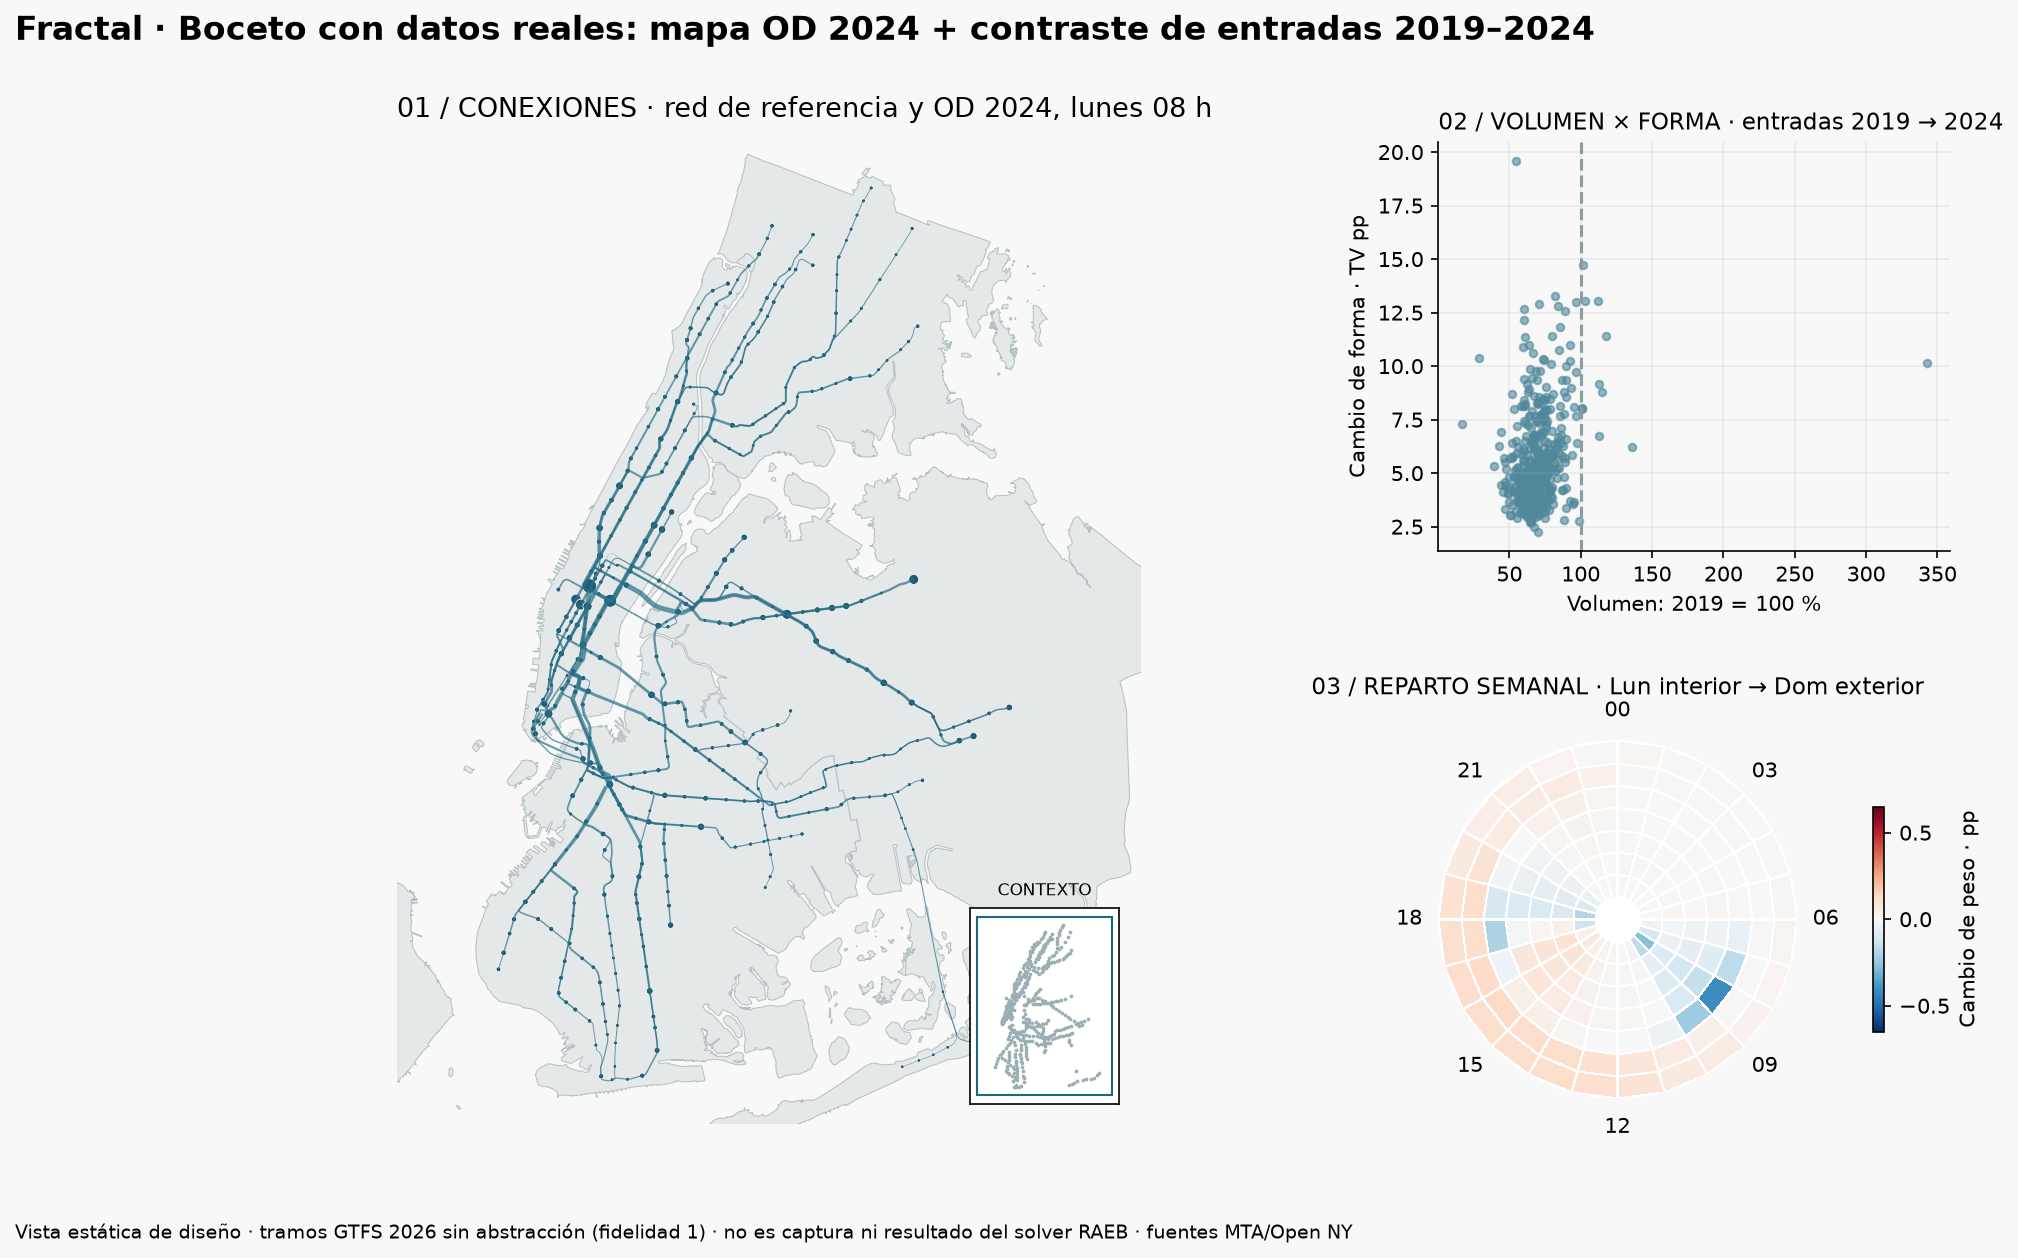
\includegraphics[width=.92\textwidth]{panel-actual.png}
\caption{Boceto estático basado en datos reales. Mapa de tramos GTFS con carga asignada de la cohorte lunes 08 h de 2024; dispersión y reloj de entradas 2019--2024. Representa fidelidad 1, no una captura del solver ni una evaluación de interacción.}
\end{figure*}
\section{Resultados preliminares}
La Tabla~\ref{tab:territory} usa entradas de todos los meses y semanas estandarizadas. El Bronx conserva 58,4\% del volumen de 2019 y pierde 1,44 pp de participación. Brooklyn pierde volumen absoluto pero gana participación del sistema: ambas dimensiones deben separarse.
\begin{table}[h]\centering\small
\begin{tabular}{lrrr}\toprule
Borough & Índice & $\Delta$ cuota & TV pp\\\midrule
Bronx & 58,4\% & $-1,44$ pp & 1,88\\
Brooklyn & 72,1\% & $+0,37$ pp & 4,60\\
Manhattan & 71,3\% & $+0,27$ pp & 4,71\\
Queens & 75,0\% & $+0,81$ pp & 3,32\\\bottomrule
\end{tabular}\caption{Entradas: 2024 frente a 2019. Índice base 100; TV de perfiles territoriales agregados.}\label{tab:territory}
\end{table}
En OD, la participación de Manhattan entre los destinos desde Brooklyn pasa de 42,07\% en 2021 a 46,71\% en 2024; desde Queens, de 47,09\% a 50,30\%; desde Bronx, de 53,53\% a 57,22\%. Esto describe composición, no prueba motivos de viaje ni disminución absoluta de viajes locales. Las tablas completas y las muestras para cada tarea son reproducibles mediante \texttt{prepare\_analytical\_tasks.py}, con SHA y controles.
\section{Discusión, evaluación y límites}
Se conserva el registro original de crítica; instrucciones posteriores del usuario explican el panel único, el reloj principal, los parámetros y la ausencia de reproducción. No se fabrican evaluadores ni resultados de uso. Las pruebas técnicas cubren estructura, separación de fuentes, balance y componentes numéricos; la evaluación con la audiencia y auditoría completa de accesibilidad siguen pendientes.
La red 2026 no reconstruye el servicio 2019--2024 y minimiza distancia sin horarios, esperas ni compatibilidad temporal de patrones. El OD es estimado y su hora corresponde a inicio, no presencia simultánea en un segmento. No medimos capacidad o congestión. Un origen de metro no identifica residencia ni un destino empleo o turismo. Los años completos no controlan toda estacionalidad y no permiten atribuir causalidad a pandemia o teletrabajo.
\section{Trabajo futuro y conclusión}
El panel principal y el contraste histórico están implementados. Las seis tareas tienen evidencia tabular; faltan integración de síntesis territorial, balance y consulta exacta por tramo, detector de ventanas y escenario interactivo. El plan propone responsables y fechas para ratificar con el equipo. No se confunden estos pendientes con funciones terminadas.
El caso muestra por qué volumen, participación territorial y composición temporal deben analizarse conjuntamente. El valor está en formular estudios mejor localizados y verificables; la utilidad perceptual y operacional todavía requiere evaluación.
\begin{thebibliography}{9}
\bibitem{raeb} W. Zeng et al., ``Route-Aware Edge Bundling for Visualizing Origin-Destination Trails in Urban Traffic,'' CGF 38(3), 581--593, 2019. doi:10.1111/cgf.13712.
\bibitem{kdeeb} C. Hurter, O. Ersoy y A. Telea, ``Graph Bundling by Kernel Density Estimation,'' CGF 31(3pt1), 865--874, 2012. doi:10.1111/j.1467-8659.2012.03079.x.
\bibitem{clock} M. Dhont et al., ``Visual Analytics for Extracting Trends from Spatio-temporal Data,'' LNCS 12588, 122--137, 2020. doi:10.1007/978-3-030-65742-0\_9.
\bibitem{tv} J. Fredriksson y A. Karlström, ``A Fully Neural Network-Based Travel Demand and Scheduling Model, Covering Activities, Destinations, and Modes of Transportation,'' Data Science for Transportation 7, 28, 2025. doi:10.1007/s42421-025-00141-5.
\bibitem{tasks} M. Brehmer y T. Munzner, ``A Multi-Level Typology of Abstract Visualization Tasks,'' TVCG 19(12), 2376--2385, 2013. doi:10.1109/TVCG.2013.124.
\bibitem{comparison} M. Gleicher et al., ``Visual Comparison for Information Visualization,'' Information Visualization 10(4), 289--309, 2011. doi:10.1177/1473871611416549.
\bibitem{mantra} B. Shneiderman, ``The Eyes Have It: A Task by Data Type Taxonomy for Information Visualizations,'' IEEE VL, 336--343, 1996. doi:10.1109/VL.1996.545307.
\bibitem{data} MTA, Open NY hourly ridership and OD estimates; official dataset IDs and GTFS snapshot in the reproducibility manifests. NYC DCP, borough and NTA 2020 boundaries.
\end{thebibliography}\end{document}
